\documentclass[12pt, letterpaper]{article}
\usepackage[margin=1in]{geometry}
\usepackage{graphicx}
\graphicspath{ {figures_EC102/} }

\title{EC102 Revision}
\author{Cedric Tan}
\date{April 2019}

\begin{document}
\maketitle
\abstract{

This is a review of macroeconomic lectures by Franceso Caselli in Lent Term of 2019. The notes are mine fully and may not be authentic to the lecturer's as they have been modified.

The format of this material is usually recounted slide by slide but some slides may be merged together as the material fits appropriately with one another.
}

\newpage
\tableofcontents
\newpage

\section{Introduction to Macro}
Macroeconomics is about the performance of the economy overall. Topics that will be covered in this course are as follows:
\begin{itemize}
	\item Long-run Economic Growth
	\item Booms and Recessions
	\item Inflation and Deflation
	\item Unemployment
	\item Financial, Currency and Sovereign Debt Crises
\end{itemize}

Further to that, here are some of the big macroeconomic issues that we are facing today in (\textbf{April 2019:})
\begin{itemize}
	\item Why are we growing so slowly and is the slowdown permanent?
	\item What are the consequences of \textbf{Brext} for UK growth?
	\item Has austerity been a good idea? In the UK? In the Eurozone?
	\item Why is inflation so low and what should Central Banks do about it?
	\item What will happen when Central Banks end \textbf{Quantitative Easing?}
	\item Will lower-income countries ever catch up to the high-income ones?
	\item Will there be a financial crisis in China?
	\item Have we done enough to prevent a new financial crisis?
\end{itemize}

\begin{center}
	\textbf{Colin O'Shea:} \textit{Market sentiment always dictates what will happen. Policy implementation may not always work as it is dependent on sentiment.}
\end{center}

\begin{center}
	\Large{\textbf{Welcome to macroeconomics}}
\end{center}

\newpage
\section{Economic Growth}
We will begin with a definition of Economic growth:

\textit{It is the \textbf{long run} changes in \textbf{material living standards.} \\}

Long run means:
\begin{itemize}
	\item Persistent changes over time
	\item One generation compared to the previous
	\item Definitely not a quarter by quarter analysis \\
\end{itemize}

Material means:
\begin{itemize}
	\item Food, housing: these are \textbf{physical objects}
	\item Education, healthcare
	\item Income to access these goods and services
\end{itemize}

\subsection{Preliminary Questions on Growth}
Further to this, we will ask some preliminary questions on growth to get the gears running:
\begin{itemize}
	\item How do we measure it?
	\item Is indefinite growth feasible? i.e. \textbf{Growth forever on an upwards trend?}
	\item Is indefinite growth even desirable or \textbf{even a good idea?}
\end{itemize}

\subsection{Measuring Growth}
We will begin the discussion on growth by looking at various ways of measuring it

\subsubsection{Measuring Growth: GDP per Capita}
Definitions:\\
\textbf{GDP:} the value of all goods and services produced by an economy in a year \\
\textbf{per Capita:} divided by the total population \\

This indicates that everyone gets an equal share of the pie \textit{which might not necessarily be the case hence the doubt about the measure.} \\
But it does provide an idea of the \textbf{standard of living within the society} \\
\begin{center}
	The common consumption method of measuring GDP is:\\
	$GDP = AD = C + I + G + (X-M)$
\end{center}

\subsubsection{Measuring Growth: Median Income}
Definitions:\\
\textbf{Median income:} the level of income at which 50\% of the population is above and 50\% of the population is below.\\

This gives a rough indication of the income distribution within a country, something that \textbf{GDP per Capita} does not show. This can be adjusted for family size as well.
\begin{center}
	In the UK, for example:
	\begin{itemize}
		\item Median: £27,300
		\item Average: £27,600
	\end{itemize}
\end{center}

\subsubsection{Measuring Growth: Multi-dimensional}
Further to the previous two measures of growth which are strictly numerical, we can adopt multi-dimensional measures of growth as well. These are considered holistic approaches to measurement. Examples include:
\begin{itemize}
	\item \textbf{The Stiglitz Commission:} a dashboard approach which measures a whole host of indicators such as health, education and politican voice
	\item \textbf{United Nations HDI:} a measure for GDP per Capita, education through literacy rates and mean years of schooling and life expectancy
	\item \textbf{Utility-based Index:} measures happiness through indicators such as  consumption, life expectancy, inequality and leisure
\end{itemize}

\subsubsection{Measuring Growth: Depletion}
Another method to measuring growth is simply through depletion. \\
This means \textbf{we measure not what we build} but rather \textbf{what we have depleted in the process of building it.} This measure is an innovative way of seeing growth due to the economic problem of scarcity.

\subsubsection{Focus on Growth}
Concerning other factors such as education, life expectancy and so on, it is usually okay for us to \textbf{focus on growth} as there is a positive correlation with all the other measures:
\begin{itemize}
	\item Over long periods of time
	\item Over countries with very different living standards
\end{itemize}
It simply provides a standardised measure which does not need to take in subjective accounts to be fully effective. The limitations it has can be supported by the holistic measures mentioned.

\subsection{Sustainability and Desirability of Growth}
Here we will discuss the sustainability of growth and whether or not an indefinite growth path is desirable in the first place.

\subsubsection{Problem 1: Running out of resources}
The issue is self-explanatory, when we begin to run out of natural resources, the growth trend will gradually plateau and then dip if we are unable to continue producing. Presented below are key solutions to the issue:
\begin{itemize}
	\item \textbf{Substitution:} finding alternative solutions e.g. renewable energy rather than fossil fuels
	\item \textbf{Efficiency:} becoming better at using less or the equal amount for more e.g. mileage on a car has become much more efficient
	\item \textbf{Recycling:} reusing old unused materials again for production e.g. plastics, card etc.
\end{itemize}
Further to that, we have to recognise the role of the market and the role of public policy:
\begin{itemize}
	\item Role of the market:
		\begin{itemize}
		\item Spontaneity of market solutions that arise
		\item Innovation from an incentive to profit
		\item Creation of efficiency gains to capture a wider market share
		\end{itemize}
	\item Role of public policy:
		\begin{itemize}
		\item Promotion of sustainable growth
		\item Use of regulation e.g. carbon caps or subsidies to promote to disincentivise or promote certain market practices.
		\end{itemize}
\end{itemize}

\subsubsection{Problem 2: Environmental Degradation}
Environmental degradation and climate change are key issues that might affect our ability to grow. These are due to the issues cause by them that hinder economic growth such as weather patterns affecting our agriculture. \\
These are due mainly to externalities which:
\begin{itemize}
	\item Arise when agents engage in activities which have an \textbf{impact on others} but has \textbf{no market} as the price adjustment mechanism is non-existent
	\item Have an effect on a third party during the \textbf{consumption or production} of a good or service
\end{itemize}
The technical solutions mentioned above are still key to resolving these issues but:
\begin{itemize}
	\item Externalities are only easier to control at a local and national level
	\item Global externalities, which cause the most issues, is where the difficulty lies as \textbf{coordination across governments} is required but not guaranteed. \textit{Trump and pulling the USA out of the Paris agreement is a good example.}
\end{itemize}

\subsubsection{Is growth even a good thing?}
Here is a proposal: \textbf{Zero Growth in rich countries.} This will allow us to:
\begin{itemize}
	\item Have more leisure as there is no need to work
	\item Focus on what matters such as relationships, relaxation and pursuit of alternative activities such as your hobbies
\end{itemize}

But here are some pro-growth arguments to counter those above:
\begin{itemize}
	\item Quantity of life is greater due to a \textbf{longer life expectancy}
	\item Periods of low growth lead to nasty politics: avoid this by not advocating for a \textbf{Zero Growth} policy
\end{itemize}

So perhaps we can leave the no-growth option as an individual one. You choose yourself if you want to pursue this path but it should not be one that society as a whole adopts.

\subsection{Economic Growth: Appendix}
Find related materials here 
\subsubsection{Formulae and Definitions}
\begin{itemize}
	\item \textbf{Growth Rate:}
		\begin{itemize}
			\item Change is the new level divided by the initial level
			\item \textbf{Formula:} $\frac{GDP_{T2} - GDP_{T1}}{GDP_{T1}}$
		\end{itemize}
\end{itemize}

\subsubsection{Figures}

\begin{figure}[h]
\centering
	\begin{minipage}{0.45\textwidth}
		\centering
		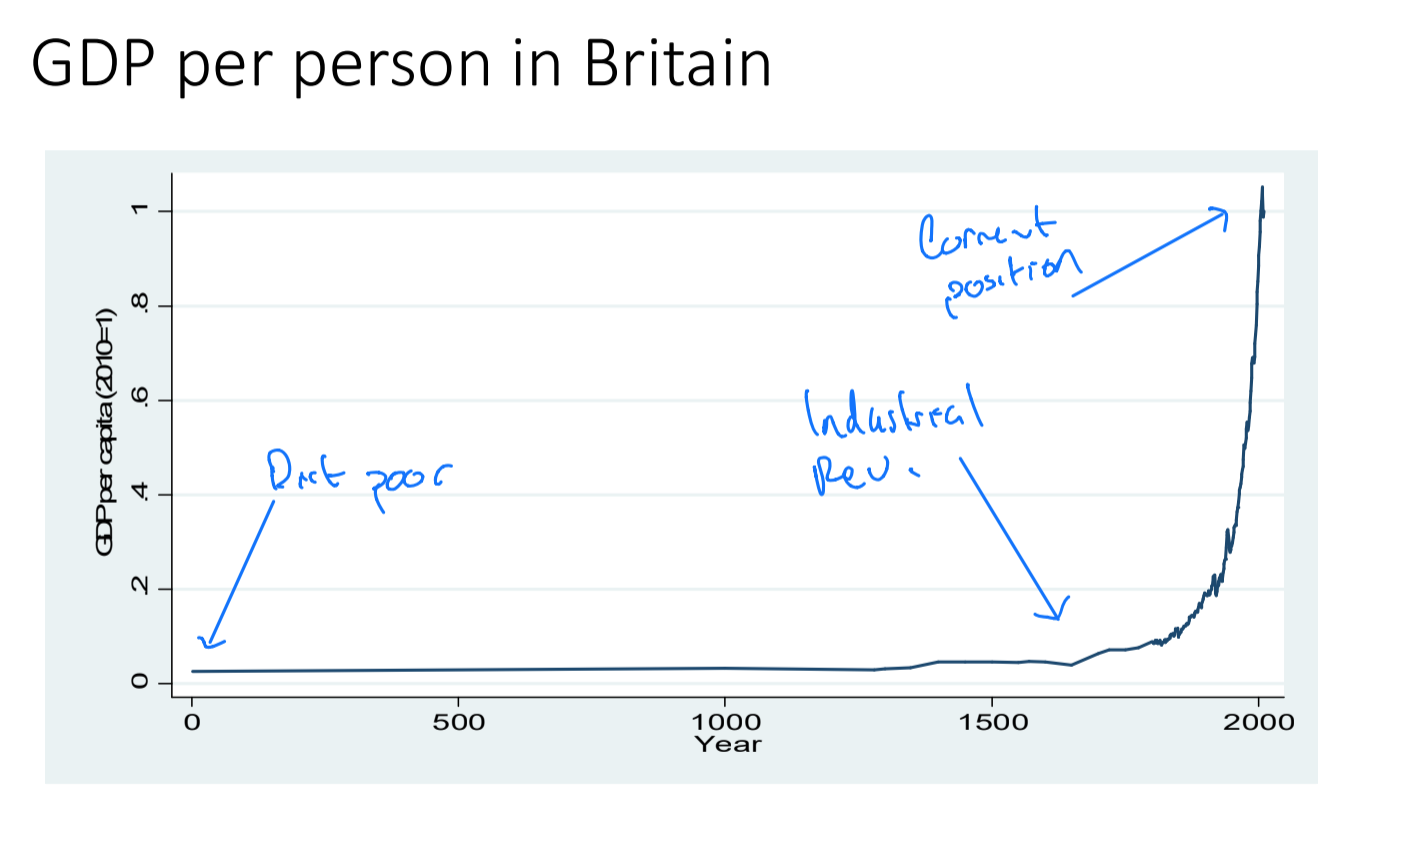
\includegraphics[width=.7\textwidth]{britain_gdp_1}
		\caption{Britain's GDP over time}
		\label{fig:britain_gdp_1}
	\end{minipage}\hfill
	\begin{minipage}{0.45\textwidth}
		\centering
		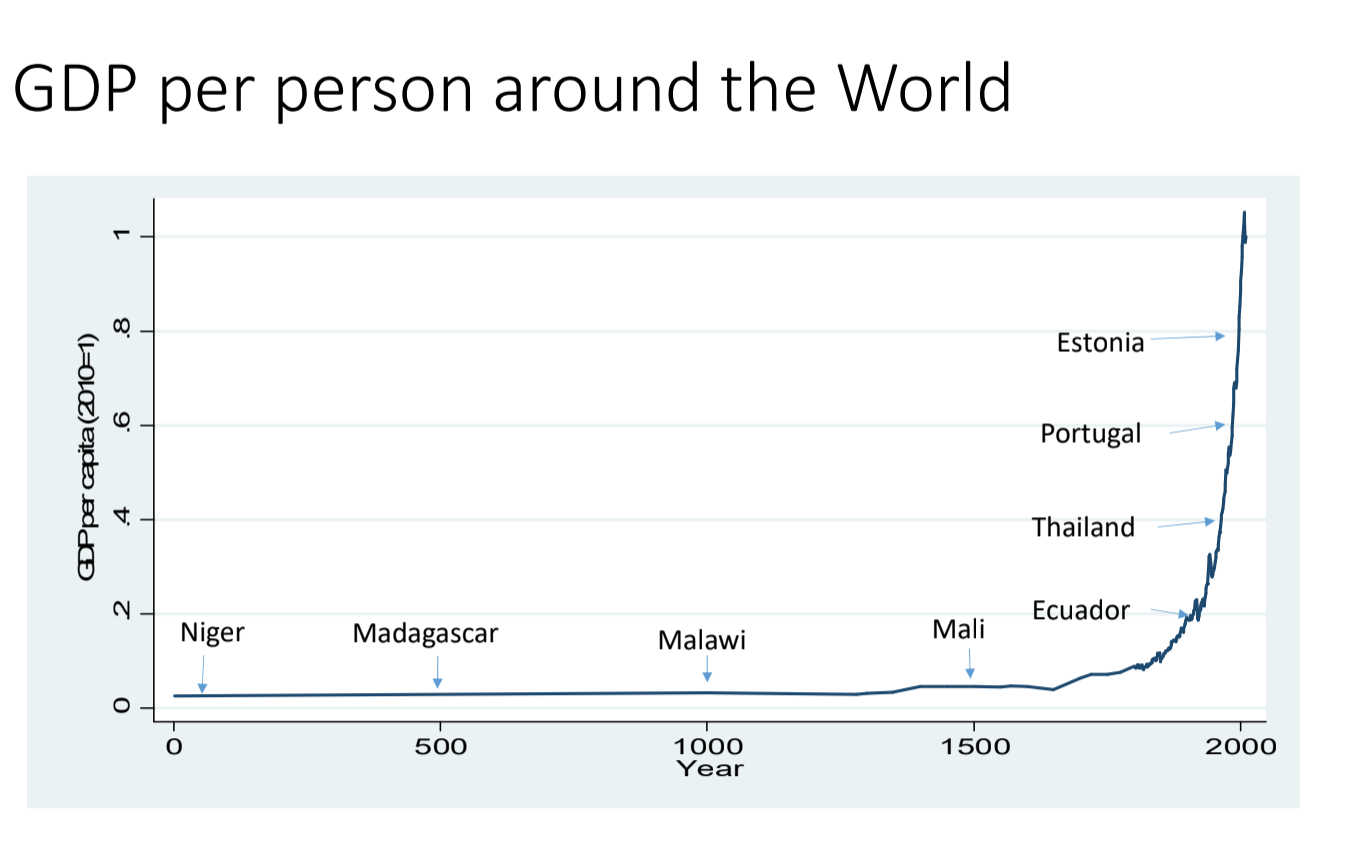
\includegraphics[width=.7\textwidth]{britain_gdp_2}
		\caption{Britain's GDP compared to other countries NOW}
		\label{fig:britain_gdp_2}
	\end{minipage}
\end{figure}	
	
\begin{figure}[h]
	\begin{minipage}{.45\textwidth}
		\centering
		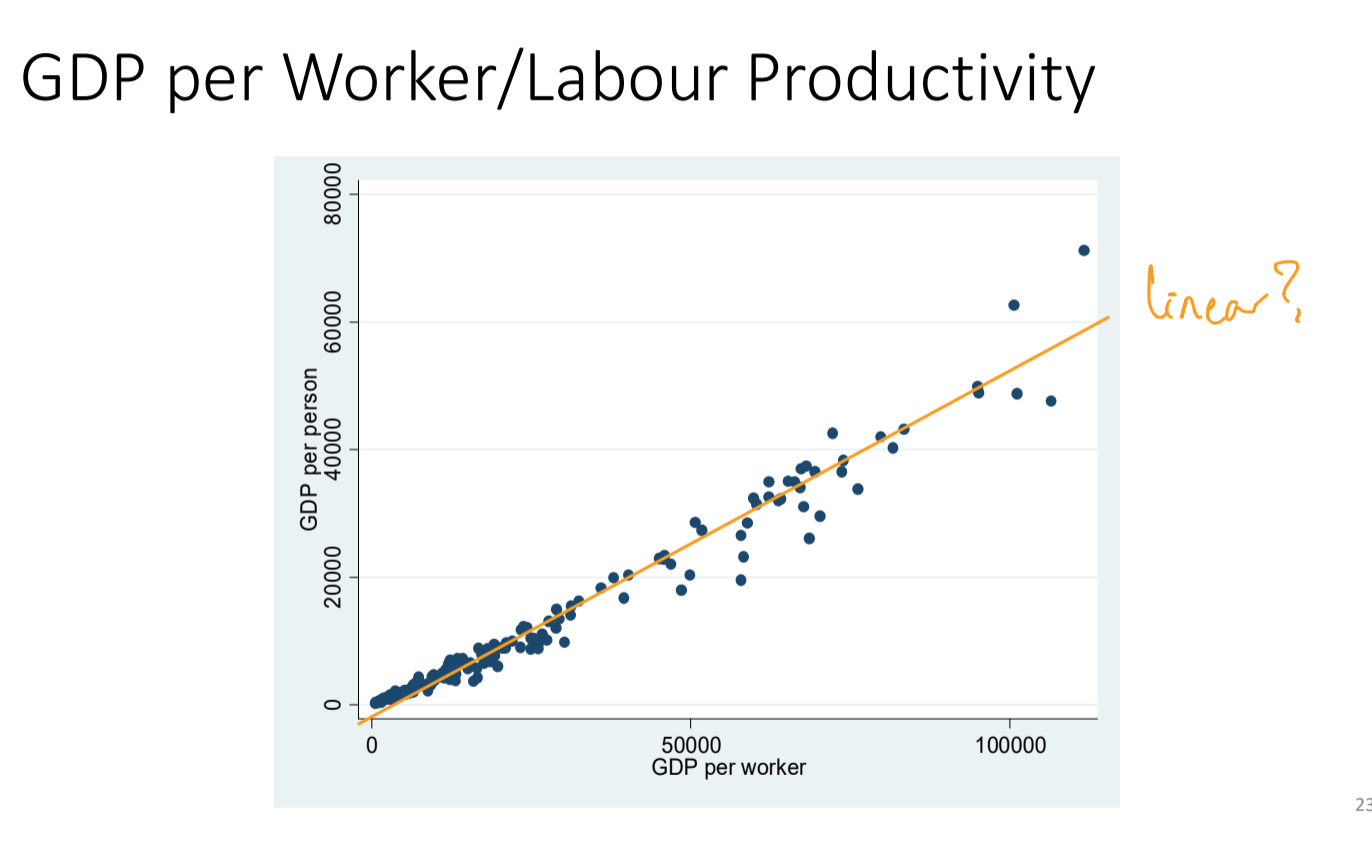
\includegraphics[width=.7\textwidth]{gdp_productivity_1}
		\caption{GDP vs Productivity}
		\label{fig:gdp_productivity_1}
	\end{minipage}\hfill
	\begin{minipage}{.45\textwidth}
		\centering
		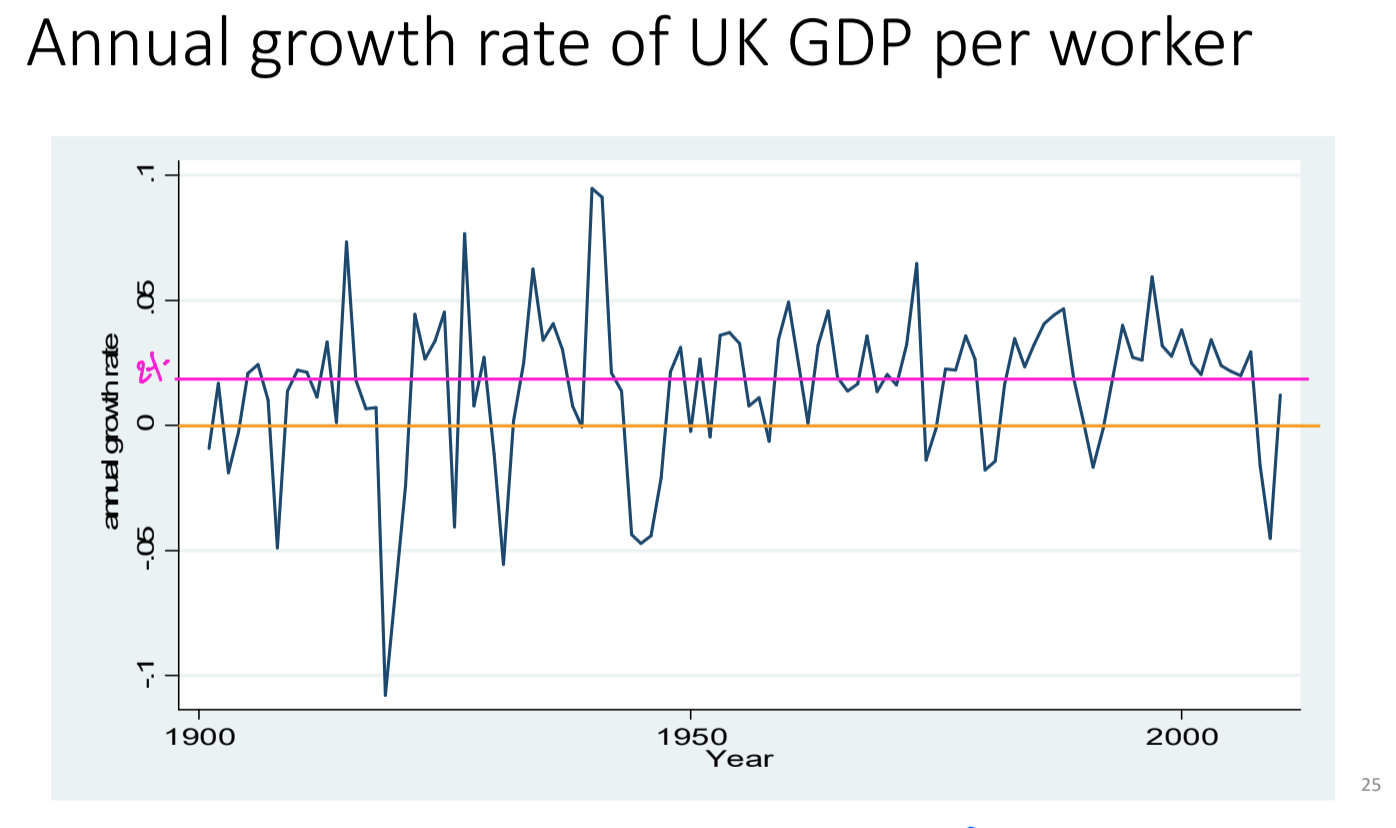
\includegraphics[width=.7\textwidth]{britain_gdp_3}
		\caption{Britain's GDP Growth Trend}
		\label{fig:britain_gdp_3}
	\end{minipage}
	
\end{figure}

\newpage
\section{Growth Engines}
Here we move onto the main drivers for growth in the economy. We will use an analogy of a hunting village, whereby the hunters use arrows to catch their game, to spell out these engines specifically. The engines that we will discuss are as follows:
\begin{itemize}
	\item More arrows per hunter: \textbf{Capital Accumulation}
	\item Better arrows to use: \textbf{Technological Change}
	\item Hunting in a pack: \textbf{Management Quality}
	\item More hunting training: \textbf{Human Capital Accumulation}
\end{itemize}

\textbf{n.b. For this example, we will assume that $Kills/worker = GDP/capita$ and $Kills \; Total = GDP \; Total$}

\subsection{Capital Accumulation}
More arrows per hunter in our analogy is called \textbf{capital} accumulation as we have more productive resources to utilise in our day to day production of game. This is done through the process of \textbf{investment.}

\subsubsection{Definitions}
Beginning with some definitions:
\begin{itemize}
	\item \textbf{Capital:} the stock of equipment and structures at a certain point in time
	\item \textbf{Investment:} the addition toe the stock of equipment and structures
\end{itemize}

\subsubsection{Accumulation and Growth}
The causal mechanism for accumulation and then growth is through how workers use capital. 

Think of capital as \textbf{aids in production to effectively produce more,} like how the arrows in the hunting village help with killing more animals. 

Investment leads to the accumulation of this capital as there will be growth in \textbf{capital per worker,} adding to the overall stock. 

Growth in capital per worker leads to growth in \textbf{GDP per worker} as each worker is more productive.

\subsubsection{Nature of Investment}
The nature of investment is such that there is a sacrifice of current consumption to achieve a greater level of future consumption. Some of the workers and capital are labouring to produce new capital instead of producing goods and services for immediate use.

\subsubsection{Investment in an Open Economy}
We can not sacrifice consumption domestically to gain investment into the economy through the use of imports: \textbf{capital goods are imported whilst domestic workers dedicate themselves to consumption goods.}

However, this implies \textbf{debt accumulation} as you are borrowing funds to pay for these expensive imported capital goods. Since foreign debt cannot be accumulated \textbf{indefinitely,} the consumption sacrifice is only postponed to a later date. This is when there is a requirement to pay off debt. Hence, \textbf{the later sacrifice} meaning that there is still a trade-off between investment and consumption.

\subsection{Technological Change}
Better arrows per hunter is called \textbf{technological change} as we have better productive resources to utilise. \textbf{Note that this does not mean more productive resources.} As we have better resources to use, we are more productive with them. Change happens through \textbf{innovation.}

\subsubsection{Definitions}
Beginning with some definitions:
\begin{itemize}
	\item \textbf{Innovation:} introduction of new ways of doing more with less or the same amount. These efficiency gains are found in the \textbf{production process.} Innovation is usually knowledge shared freely in society.
\end{itemize}

Note that in modern economies, innovation is the outcome of:
\begin{itemize}
	\item Basic research, mostly done in universities
	\item Research and Design \textbf{(R\&D),} mostly done in firms
\end{itemize}

\subsubsection{Economics of R\&D}
There are some key characteristics of innovation that must be recognised to show the thorny parts of R\&D as it can sometimes cause barriers to technological change:
\begin{itemize}
	\item \textbf{Upfront research costs:} Increase the burden of risk as there is a large requirement of upfront capital.
	\item \textbf{Non-Rivalrous:} One person's use does not exclude another person from using it. This means that if one firm creates an idea, without any protection around it, another firm can steal the idea and use it.
\end{itemize}
Hence, without any intervention, the costs for R\&D are too high whilst the benefits are too low. We can see that with an equation below:
\begin{center}
$N = Net\;Benefit$ \\ $R = Reward\;for\;Successful\;R\&D$ \\ $P_R = Probability\;of\;Success$ \\ $C = Cost\;of\;R\&D$ \\ $P_C = Probability\;of\;Idea\;Stolen$
\end{center}
Hence knowing that $P_R$ is low and $P_C$ is high, we have the equation:
\begin{center}
$N = R \times P_R - C\times P_C$ where $N<0$
\end{center}

\subsubsection{Policy Solutions to the R\&D Problem}
Here are some solutions:
\begin{itemize}
	\item Patents:
		\begin{itemize}
			\item Intellectual property rights
			\item Effective creation of monopolies over a certain good or service
			\item Usually lasts 15-20 years
			\item Opportunity for firms to make profit from their R\&D
		\end{itemize}
	\item Subsidies: reduced costs for R\&D ventures conditional on their R\&D performance
\end{itemize}

\subsubsection{Economics of Basic Research}
Basic research is about the type of activity generating positive externalities, \textbf{that is, a positive effect on a third party during the production or consumption of a good or service, in this case \textit{research}.}

In terms of the funding:
\begin{itemize}
	\item Subsidies are given by the government e.g. Economic and Social Research Council (ESRC)
	\item Stimulates research and research proposals
	\item Adds value to the economy without the pricing mechanism in place effectively 'shifting the frontiers of what is possible.'
\end{itemize}

\subsubsection{Technological Change in Poorer Countries}
Imitation makes a lot more sense than innovation in poorer countries. However, the issue is that \textbf{knowledge does not flow that easily.} Limited knowledge leads to a lack of accessibility. Successful imitation, however, shows miraculous levels of growth: \textbf{China and Japan being notable examples}

This issue of information dissemination is because new ideas contain two types of knowledge:
\begin{itemize}
	\item \textbf{Explicit Knowledge:} formulas, blue prints, instructions
	\item \textbf{Tacit Knowledge:} nuanced knowledge like application with certain people etc. which cannot be communicated as effectively.
\end{itemize}

\subsubsection{Sources of International Technology Diffusion}
There exists two main ways of technological change moving around the world:
\begin{enumerate}
	\item Foreign Direct Investment
	\item Trade
\end{enumerate}

\textbf{Foreign Direct Investment (FDI):}
\begin{itemize}
	\item Foreign entity starts or acquires productive resources outside their home country
	\item Direct technology transfer through a literal implementation of the firms technology abroad
	\item Diffusion through imitation clusters, when the technology from an initial investment is taken up by aspiring entrepreneurs
	\item Competition with local, inefficient firms who need to learn/imitate/adapt or be pushed out of the market due to being priced out
\end{itemize}

\textbf{Trade:}\\
In trade there are exports and imports. Both contribute to technology diffusion:
\begin{itemize}
	\item Imports:
		\begin{itemize}
			\item Embodied technology e.g. importing IT systems
			\item Pressure on local inefficient firms to adapt $\rightarrow$ same as FDI
		\end{itemize}
	\item Exports:
		\begin{itemize}
			\item Learning by exporting $\rightarrow$ learn to be more efficient and learn how to adapt to the demands of countries abroad
			\item Market size increases $\rightarrow$ access to a larger market allows for diffusion of technology into developing countries simply because of broader exposure
		\end{itemize}
\end{itemize}

\subsubsection{International Tech Diffusion and IPRs}
\textbf{Question:} Should poorer countries enforce intellectual property rights (IPRs) of rich-country firms?\\
There is a temptation to believe that not enforcing them can lead to cheap production by imitation however possible problems persist:
\begin{itemize}
	\item It discourages FDI as there is no more profitability for these foreign firms to come into the developing market
	\item There would be adverse effects on rich country innovation as there is no longer an incentive to innovate. \textit{This is based on the premise that firms are innovating to conduct FDI}
	\item Rich countries simply do not like it. This might result in a lack of trade and a souring of international relations which can subsequently cause a trade war
\end{itemize}

Yet, even with enforcement, a lack of enforcement could persist anyway due to the negligence of IPRs and Patents in developing countries. Hence, the issue appears to be much more complicated than black or white.

\subsubsection{Embodied Technology}
The distinction between capital accumulation or growth and innovation or imitation is conceptually useful. \textbf{However,} in practice, a lot of innovation or imitation is embodied in capital itself. Thus, the two often come in the same package. Investment is itself a source of technological change.

\subsection{Management Quality}
Management quality drives growth through putting people who are good at the right thing in the right place. This is done through \textbf{specialisation} and \textbf{comparative advantage.} Examples of high management quality:
\begin{itemize}
	\item Adam Smith's pin factory $\rightarrow$ division of labour (specialisation)
	\item Henry Ford's assembly line $\rightarrow$ division of labour as well
	\item Outsourcing and global supply chains $\rightarrow$ utilising comparative advantage
	\item Gig economy $\rightarrow$ workers connecting through an information supply chain with an increased division in labour and level of specialisation
\end{itemize}

\subsubsection{Definitions}
Beginning with some definitions:
\begin{itemize}
	\item \textbf{Specialisation:} focusing on one task and increasing the efficiency at which it is done.
	\item \textbf{Comparative Advantage:} whereby the opportunity cost to produce something for something else/someone is less than another entity. \textit{One would say that a country has a comparative advantage if its opportunity cost to produce is less than another's.}
\end{itemize}

Further to that, organisational change can sometimes come as a form of technical change. You can do more with the same resources and it often requires some upfront R\&D investment. An example would be something like \textbf{software to manage supply chains,} both organisational and technical.

\subsubsection{The Indian Manufacturing Case Study}
To test the real effects of management quality, consulting companies went into India to perform a test whereby control groups of firms were given no management consultants while tested firms were given management consultants to fix their most pressing issues over a few days.

\textbf{Before:}
\begin{itemize}
	\item The manufacturing firms in India were very disorganised with dirty and poorly maintained machinery whilst equipment was lying across the floor. 
	\item Yarn had no labels, order or damp protection. Further, it was piled so high, access was restricted in the factory itself
	\item Poor storage practices also made some stock unusable, requiring further treatment to be used again
\end{itemize}
\textbf{After:}
\begin{itemize}
	\item Stock was organised and labelled
	\item Stock was also tagged and entered into the computer
	\item Factory was cleaned and maintained to a higher standard
\end{itemize}

\subsubsection{Managerial Quality}
Within a country, there is a big disparity in productivity among firms possibly due to the differences in managerial quality as a result of the different levels of organisation. There would be big gains from bringing up efficiency at the tail: \textit{the lower end of the distribution is lagging far behind but can account for a lot of firms within the country.}\\

\textbf{Causes of Poor Managerial Quality:}
\begin{itemize}
	\item Dynastic Management: management of the firm kept within a family, not meritocratic and there is no guarantee of skill or will from future generations
	\item Crony Capitalism: Prevalent in low-income countries. Owners and managers are kept in a tight circle and benefits are accrued through political connections.
		\begin{itemize}
			\item Shareholders can benefit due to their own connections
			\item Productivity will be low due to mostly incapable management $\rightarrow$ again, not meritocratic but based on nepotism
		\end{itemize}
	\item State Owned Enterprises: directly appointed by the government, low productivity due to failed selection process at some points\\
\end{itemize}

\textbf{Entry Costs, Financial markets and Managerial Quality}
\begin{itemize}
	\item Talented outsiders could:
		\begin{itemize}
			\item Buy out incumbents $\rightarrow$ but a lack of capital means they might not be able to, further, they can't judge their own talent compared to the market without experience
			\item Enter with their own startups to compete them out of the market
		\end{itemize}
	\item High entry costs:
		\begin{itemize}
			\item Upfront production costs as capital raising is difficult
			\item Licenses, permits etc. are barriers to entry
		\end{itemize}
	\item Poorly developed financial markets:
		\begin{itemize}
			\item Typically as a result of inefficient contract enforcement
			\item This adds further difficulty to ensuring capital
		\end{itemize}
\end{itemize}
Hence, it is obvious that Managerial Quality can be severely affected by a plethora of other factors. However, its contribution to growth can also be very large, especially at the weaker end of the distribution where basic practices - \textbf{ref: Indian Case Study} - have not even been implemented.

\subsection{Human Capital Accumulation}
More years in hunting school in our analogy translates to human capital accumulation. With more human capital, workers are intrinsically more productive and efficient and can apply their knowledge to technological, capital and managerial change. This is a cumulative effect from education that has knock-on effects on the facilitation of innovation and imitation.

\subsubsection{Definitions}
Beginning with some definitions:
\begin{itemize}
	\item \textbf{Human Capital:} anything embodied in workers which makes them more productive, a form of internal development
\end{itemize}
The greatest focus of policy thus far has been \textbf{schooling} and \textbf{health} which aim to improve a persons ability to live and participate in the economy. Examples of foundations that have helped to develop this are:
\begin{itemize}
	\item The Gates Foundation who aid in Malaria efforts and education
	\item The United Nations who have committees dedicated to raising the standard of living through education and healthcare especially in underdeveloped countries
\end{itemize}

\subsection{Engine Interaction}
We will discuss here how these growth engines interact and whether or not growth can come from a single engine. The latter first:

\begin{center}
\noindent\fbox{\begin{minipage}{.9\textwidth}

\textbf{Ten hunters, 3 permanently on arrow-making duty. Initial endowment of 1 arrow power hunter. Over time, the change in GDP per worker will:}
\begin{enumerate}
	\item Increase
	\item Decrease
	\item Stay constant
\end{enumerate}

\textbf{\textit{Answer is 2.} Decrease due to the diminishing marginal returns on capital.} At some point, producing more capital leads to a plateauing increase in productivity.

\end{minipage}}
\end{center}

Capital accumulation and GDP growth is shown through the average product of capital. This is known by $Average\;Product\;of\;Capital = \frac{GDP\;per\;Worker}{Capital\;per\;Worker}$

In our hunting village example this would translate to $APC = \frac{Deer}{Arrows}$. Gains from additional capital is known as the marginal product of capital which is known by the additional gain to product when there is a \textbf{unit increase in capital.}

\subsubsection{Limits to Growth from Capital Accumulation}
There are definitive limits to simply using investment as a driver for growth:
\begin{itemize}
	\item The average product of capital declines due to the law of diminishing marginal returns
	\item The investment rate has a natural ceiling as it is limited by what is available i.e. it is difficult to invest beyond 100\% of GDP
	\item Capital accumulation alone cannot sustain indefinite growth
\end{itemize}
From this we can see that:
\begin{itemize}
	\item Capital accumulation depresses the average product of capital
	\item Innovation, organisational change and human capital accumulation boost the average product of capital
		\begin{itemize}
			\item Hunting in a pack improves the productivity of all arrows
			\item More trained hunters improve the productivity of all arrows
		\end{itemize}
\end{itemize}
Hence all engines appear to complement one another to ensure that one engine does not depress the average product of capital entirely.

\subsubsection{Engine Complementarity}
\textbf{Technical, organisation change and human capital accumulation keep the average product of capital falling even though capital per worker keeps increasing.}

Although they might depress their own marginal productivity, this is offset by growth in the other engines. Think of the engines as multiplicative instead of additive:
\begin{center}
	$Engine\; 1 + Engine\; 2 + Engine\; 3 + Engine\; 4$
\end{center}

\subsubsection{The Role of the State in Growth}
The State plays a major role in the growth of the economy and they can facilitate it or hinder it depending on their policy. Below are ways in which the State can impact growth:\\

\textbf{Fuel for Engines}
\begin{itemize}
	\item Investment in infrastructure which is a capital good
	\item Subsidies for R\&D and basic research
	\item Investment into education and healthcare with good policy
\end{itemize}

\textbf{Regulation}
\begin{itemize}
	\item Markets for goods and services are regulated by the state dictating what conditions people can operate under
	\item Regulation for labour and financial issues are regulated along the same lines
	\item International trade which is facilitated by the state through free trade or hindered by tariffs and trade wars
\end{itemize}

\textbf{Rule of Law}
\begin{itemize}
	\item Laws to change the operation of companies e.g. GDPR in Europe
	\item \textbf{But} rigidity is also key for smooth business operation as predictability is key to confidence in operations
	\item Implementation of processes we can follow within a reasonable boundary
\end{itemize}

\subsubsection{Corruption and Growth}
Another issue to consider when thinking about growth is corruption. Here are some reasons why:
\begin{itemize}
	\item Saps incentives for innovation, imitation and investment if corrupt officials target successful entrepreneurs. This is due to the burden of bribe payments which means less money to innovate or incentivise productivity.
	\item Creates barriers to entry for outsiders if those inside use corruption to buy protection, privileged treatment or judicial bias which means less incentive to innovate or even try in the first place
	\item Deprives government of funds for infrastructure, education, administration of justice due to embezzlement. This means less investment into the engines of growth within the economy by the government
\end{itemize}

\subsection{Growth Engines: Appendix}
Find related materials here
\subsubsection{Formulae and Definitions}
\begin{itemize}
	\item \textbf{Investment Rate:}
		\begin{itemize}
			\item A measure of the sacrifice an economy makes of current consumption for a greater level of future consumption
			\item \textbf{Formula:} $Investment\;rate = \frac{Level\;of\;investment}{GDP}$
		\end{itemize}
	\item \textbf{Average Product of Capital:}
		\begin{itemize}
			\item The amount of product that you gain from total capital invested into a worker
			\item \textbf{Formula:} $Average\;Product\;of\;Capital = \frac{GDP\;per\;Worker}{Capital\;per\;Worker}$
		\end{itemize}
	\item \textbf{$\Delta$ in Capital per Worker:}
		\begin{itemize}
			\item The change in capital that a worker has, averaged across the whole economy
			\item \textbf{Formula:} $\Delta Capital\;per\;worker = investment\; rate \times GDP\;per\;Worker$
		\end{itemize}
	\item \textbf{Growth Rate of Capital per Worker:}
		\begin{itemize}
			\item The growth in capital that a worker has, averaged across the whole economy
			\item \textbf{Formula:} $Growth\;Rate\;of\; Capital\;per\;worker = investment\; rate \times (GDP\;per\;Worker / Capital\;per\;worker)$
		\end{itemize}
		
\end{itemize}


\end{document}